\documentclass{article}

\usepackage[a4paper]{geometry}
\usepackage[ngerman]{babel}
\usepackage[utf8]{inputenc}
\usepackage[T1]{fontenc}
\usepackage{graphicx}
\usepackage{fancyhdr}
\usepackage{xcolor}
\usepackage{float}
\usepackage{hyperref}

\graphicspath{{./images/}}

\pagestyle{fancyplain}
\fancyhf{}
\lhead{\fancyplain{}{Gruppe 11 – Mathias Baumbach \& Mara Schulke} }
\rhead{\fancyplain{}{\today}}
\cfoot{\fancyplain{}{\thepage}}

\begin{document}

\begin{titlepage}
	\begin{flushleft}
		TH Brandenburg \\
		Online Studiengang IT Sicherheit \\
		Fachbereich Informatik und Medien \\
		Netzwerksicherheit \\
		Prof.\ Dr.\ Michael Pilgermann
	\end{flushleft}

	\vfill

	\begin{center}
		\Large{Einsendeaufgabe 2}\\[0.5em]
		\large{Wintersemester 2023}\\[0.25em]
		\large{Abgabetermin \today}
	\end{center}

	\vfill

	\begin{flushright}
		Gruppe 11 \\
		Mathias Baumbach (Matr-Nr. 20213703) \\
		Mara Schulke (Matr-Nr. 20215853)
	\end{flushright}
\end{titlepage}

\begin{abstract}
\end{abstract}

\tableofcontents

\listoffigures

\newpage

\section{Durchführung}

\subsection{SSL Test I}

\subsubsection*{Aufgabenstellung}

Testen Sie den Server nwsmooc.mooin.org mit der SSL-Testseite von Qualys 
und erklären Sie die Ergebnisse (hinsichtlich Zertifikaten, TLS-Versionen,
Handshakes und Details der Protokolle). Erklären Sie für eine weitere
Webpräsenz, die als "Recent Worst" bewertet wird, was bei dieser nicht stimmt. 

Hinweis: "Recent Worst" ist eine Liste auf der rechten Seite der Testseite. Zur
besseren Nachvollziehbarkeit bitte Screenshots hinzufügen. Deren Inhalte sollen
aber jeweils von Ihnen erklärt werden.

\subsubsection*{Antwort}

%\begin{figure}[H]
%	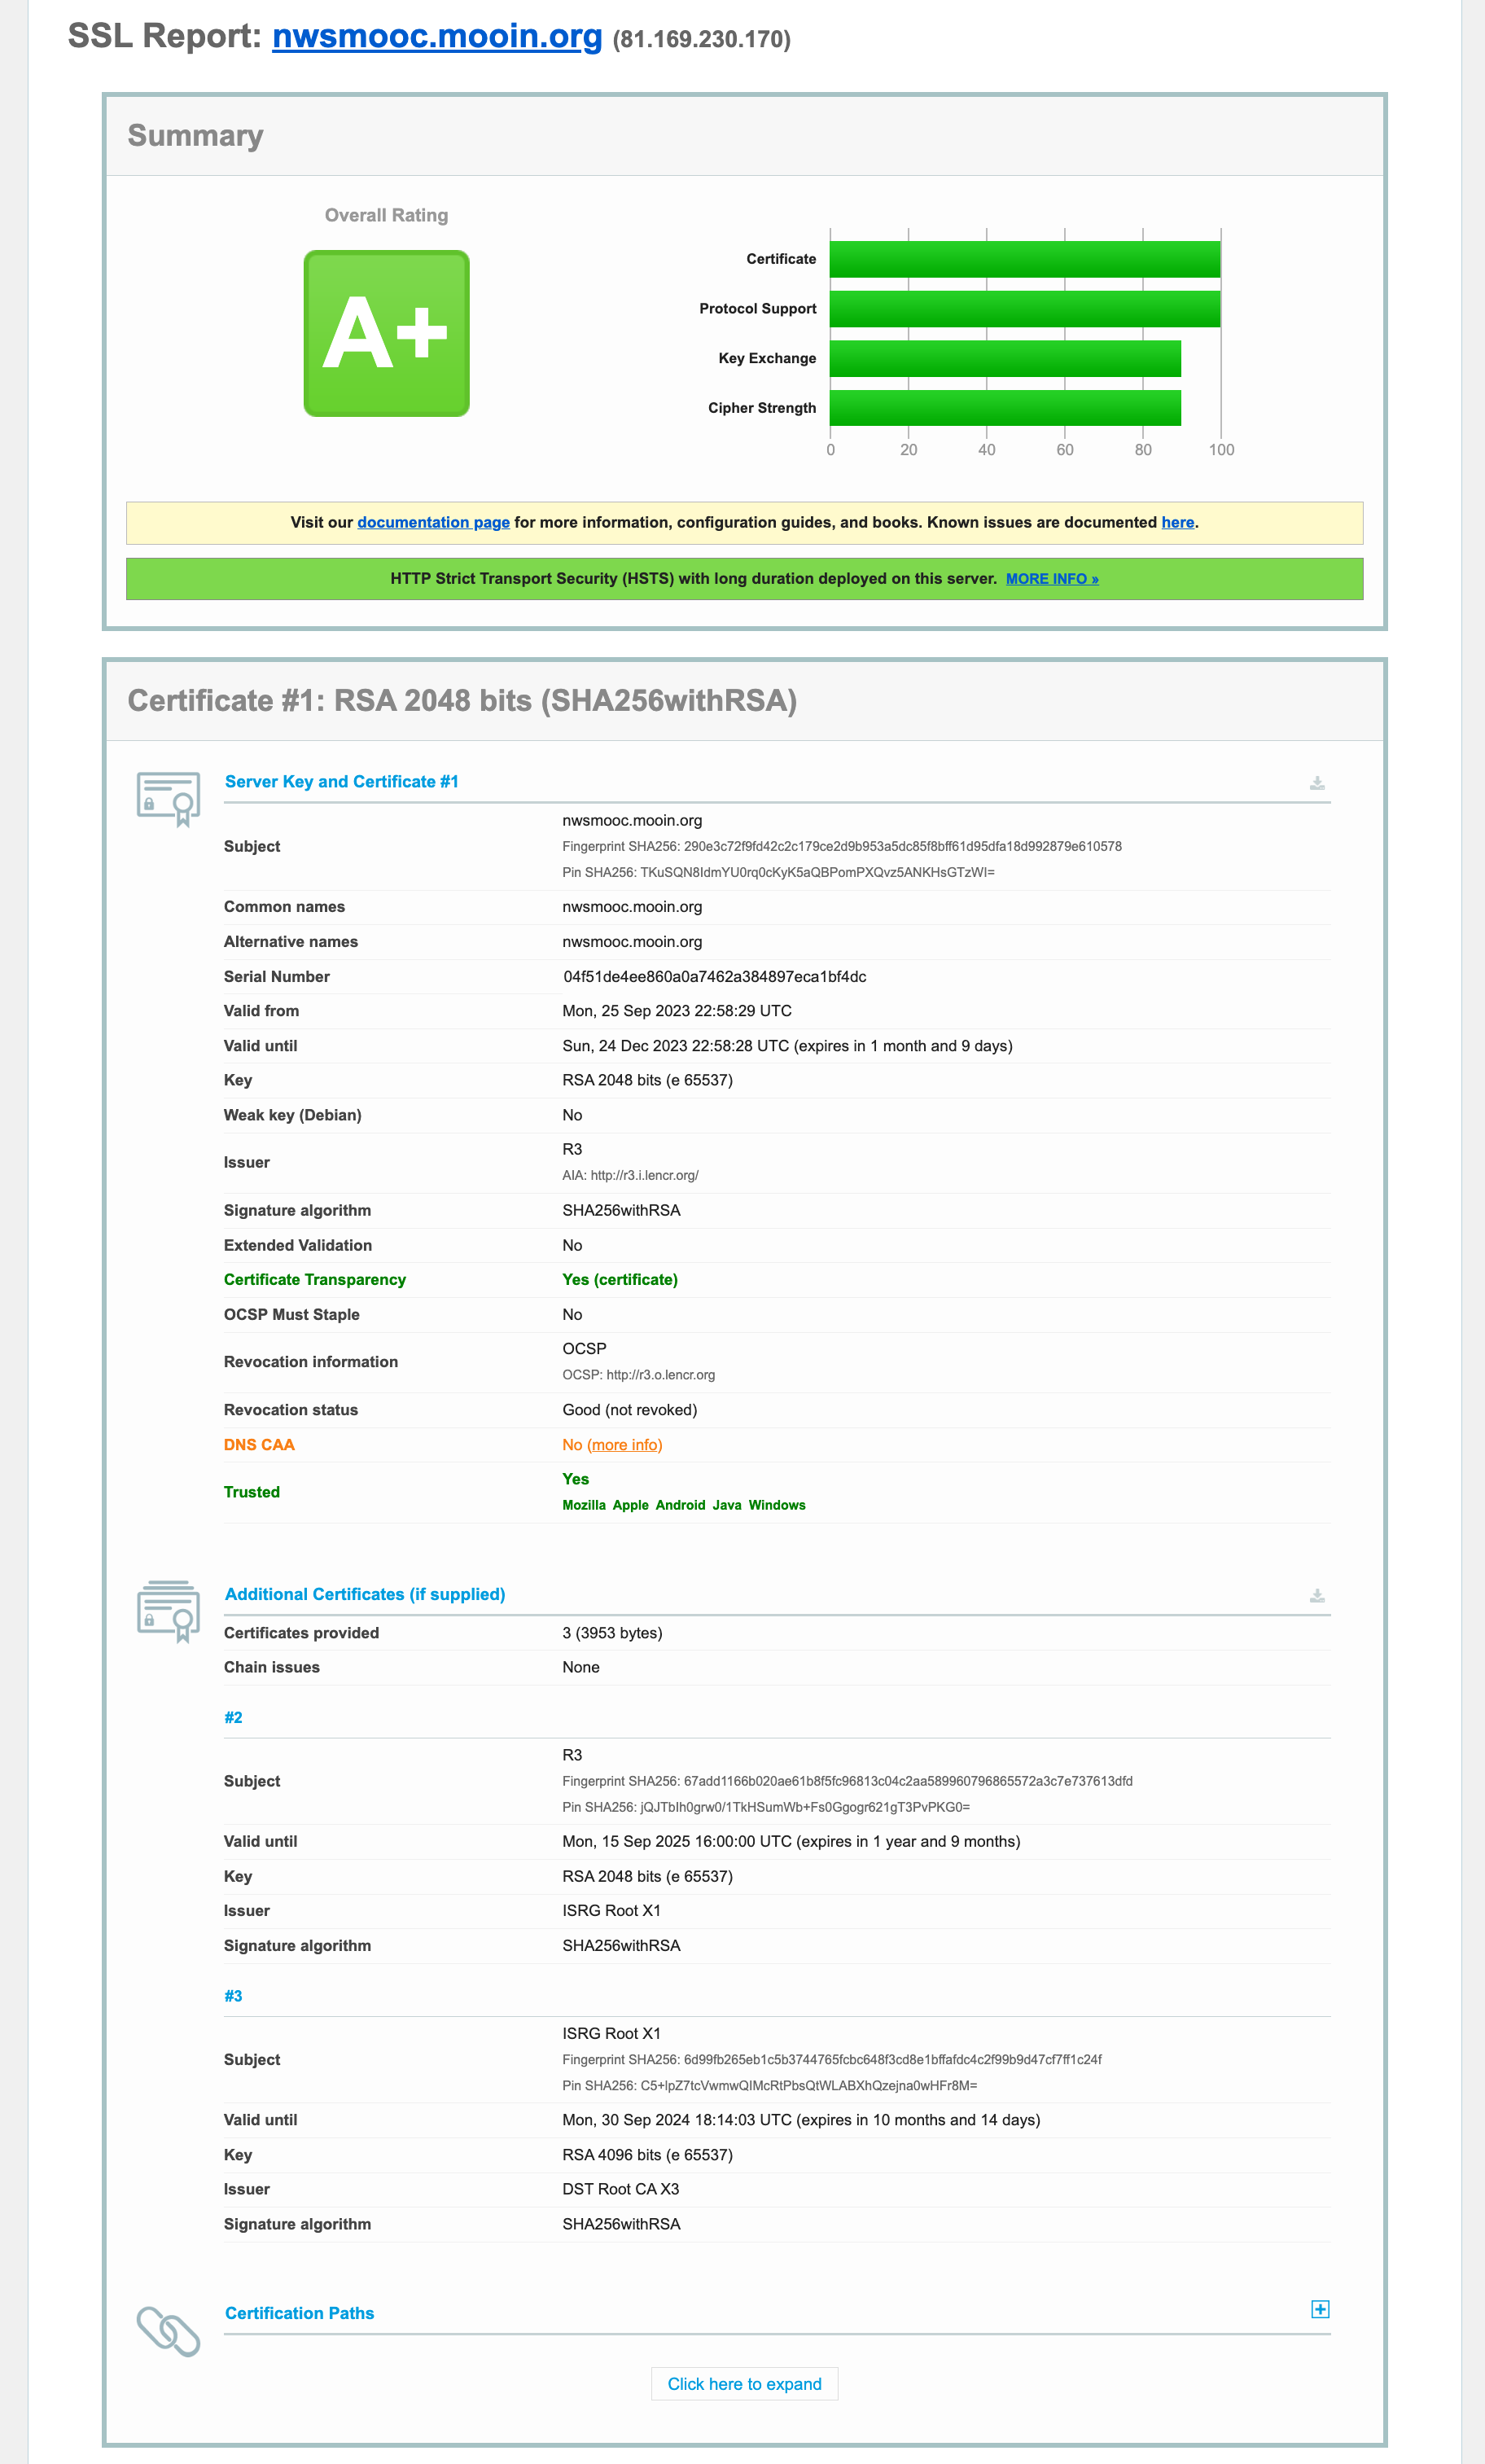
\includegraphics[width=0.75\textwidth]{images/01}
%	\centering
%	\caption{}
%\end{figure}

% https://www.ssllabs.com/ssltest/analyze.html?d=nwsmooc.mooin.org&s=81.169.230.170

https://www.ssllabs.com/ssltest/analyze.html?d=www.hoaez.com
Valid until 	Mon, 30 Oct 2023 23:00:02 UTC (expired 16 hours and 2 minutes ago)   EXPIRED
DNS CAA 	No (more info)
Trusted 	No   NOT TRUSTED (Why?)
Mozilla  Apple  Android  Java  Windows  
% → https://geekflare.com/de/dns-caa-record/
% Handshake Simulation - Chrome 49 / XP SP3 	Server sent fatal alert: handshake_failure, sonst alles grün


\newpage

\subsection{SSL Test II}

\subsubsection*{Aufgabenstellung}

Führen Sie den Client-Test von Qualys aus und erklären Sie die Ergebnisse.

\subsubsection*{Antwort}

https://clienttest.ssllabs.com:8443/ssltest/viewMyClient.html

\newpage

\subsection{SSL Test III}

\subsubsection*{Aufgabenstellung}

Rufen Sie die Testwebseiten https://aaacertificateservices.comodoca.com:442/ sowie 
https://aaacertificateservices.comodoca.com:444/  mit Firefox und mit Google 
Chrome auf. Erklären Sie, was passiert. Sind die Resultate bei allen vier Tests so 
wie erwartet?

\subsubsection*{Antwort}

\newpage

\subsection{Verschlüsselung}

\subsubsection*{Aufgabenstellung}

Installieren Sie VeraCrypt  auf Ihrem Rechner. Hierzu erhalten Sie zusätzlich eine 
VeraCrypt-Datei. In der Datei ist ein normaler und ein versteckter Container 
zu finden, die jeweils eine Datei enthalten. Das Passwort für den normalen 
Container ist der Exponent e des RSA-Schlüssels vom nwsmooc.mooin.org-Server. 
Dokumentieren Sie Ihre Vorgehensweise mit Screenshots und geben Sie 
anschließend das im versteckten Container gefundene Kennwort an.

Hinweis: Zur Bedienung von VeraCrypt können Sie sich beispielsweise hier ein Video 
ansehen: https://youtu.be/atb2pdxd394.

\subsubsection*{Antwort}

Um das zur Verfügung gestellte VeraCrypt File öffnen zu können, soll der Exponent e 
des RSA-Schlüssels der Webseite nwsmooc.mooin.org verwendet werden. Diesen 
Exponenten kann man sich ganz einfach ausgeben lassen, in dem man sich im Mozilla 
Firefox Browser jene Webseite öffnet und auf das Schlosssymbol drückt, um sich 
das Zertifikat anzusehen.

Im Abschnitt „Öffentlicher Schlüssel – Informationen“ bekommt man diesen einfach 
ausgegeben (Siehe Abbildung XXX). Wir merken an dieser Stelle an, dass wir diesen 
Exponenten zunächst auch blind getestet hatten, da in der Praxis fast immer die 
Zahl 65537 als Exponent verwendet wird. Für das RSA Verfahren werden große 
Primzahlen bevorzugt verwendet und der Algorithmus muss dabei unterschiedliche 
Operationen bei der Bearbeitung basierend auf dem Binärcode tätigen. 6553710 ist 
binär kodiert 10000000000000001 (??????????????)
was es zu einer effizienten Zahl für den Algorithmus macht (Einsen werden 
multipliziert, Nullen potenziert).

Mounted man mit VeraCrypt die bereitgestellte Datei und gibt als Passwort 65537 an, 
erhält man Zugriff auf die Datei. (siehe Abbildung XXX)


Der Inhalt des Textfiles „Datei-angezeigter-Container.txt“ lautet:	„Das 
Zugangskennwort für den versteckten Container lautet: 	VerSteCon0815“

Wir konnten uns an das Modul Digitaler Selbstschutz erinnern, in dessen Reportinhalt 
VeraCrypt bereits vorkam, und haben den Container gecloned und ein 2. Mal gemounted, 
wobei wir dieses Mal das Passwort VerSteCon0815 eingegeben haben.

Damit konnten wir Zugriff auf den versteckten Container und seinem Inhalt „Datei-
versteckter-Container.txt“ erhalten.

Der Text dieser Datei lautet:

Das gesuchte Kennwort lautet: HiddenVolumeVeraCrypt

% Die Einstellungen von SilentEye, die Sie für die Fortgeschrittenenaufgabe brauchen, 
% sind:

% Key (für beide Dateien): NWSMOOC_Test
% Passphrase (nur für jpg-Datei): SilentEye_Test

Die anderen Einstellungen entsprechen den Default-Einstellungen

Für mooin.jpg: 
Luminance Interval = 5 
Header Position = bottom
CharSet = UTF8

Für mooin.bmp (Oben beim "Media's encoding format" auf "BMP" wechseln):
Image quality: 96,975% (normal); keine Veränderungen bei "Advanced"
Aktivieren Sie zusätzlich zu "Compressed Data" jeweils auch "Encrypted Data" mit AES256. Dort muss der Key in beide Kästchen eingetragen werden.
Über die SilentEye-Aufgabe erhalten Sie über mooin.bmp übrigens schon vorab eine Aufgabensammlung zur Klausurvorbereitung.


\newpage

\subsection{Steganographie}

\subsubsection*{Aufgabenstellung}

Installieren Sie SilentEye  auf Ihrem Rechner und untersuchen Sie die 
bereitgestellten Beispieldateien. mooin.jpg enthält ein verstecktes Kennwort, 
mooin.bmp eine Datei. Die notwendigen Einstellungen können Sie der Aufgabe mit 
VeraCrypt entnehmen. Dokumentieren Sie Ihre Vorgehensweise mit Screenshots und 
geben Sie das gefundene Kennwort an.

Hinweis: Sollte es Schwierigkeiten geben, wenn Sie beide Dateien nacheinander 
untersuchen, dann schließen Sie SilentEye zwischendurch.

\subsubsection*{Antwort}

SilentEye ist eine Open-Source-Software, die zur Steganographie verwendet wird, um 
zusätzliche Informationen in Bildern und Audiodateien zu verstecken oder auszulesen. 

Um mooin.jpg zu untersuchen, öffnen wir die Datei mit dem Programm Silenteye und 
verwenden die Einstellungen aus der Lösung der Aufgabe 1.4.

Dadurch kann der verborgene Bereich des Bildes erfolgreich entschlüsselt werden und 
gibt als dekodierte Message den Text ``Kennwort: SteganographieInNWSMOOC'' frei.

Mit diesem Kennwort und den bereitgestellten Einstellungen für das zweite Bild, lässt 
sich auch dessen versteckter Inhalt sichtbar machen und entschlüsseln. Wir können an 
dieser Stelle die Datei AufgabensammlungSS16.pdf extrahieren und abspeichern.


\end{document}
